\section{Exercise 4}

Consider the C program below.
\begin{verbnobox}[\verbarg]
#include <stdio.h>
#include <stdlib.h>
#include <string.h>

int guess(char *user) {
    struct {
        int n;
        char usr[16];
        char buf[16];
    } s;

    snprintf(s.usr, 16, "%s", user);

    do {
        scanf("%s", s.buf);
        if (strncmp(s.buf, "DEBUG", 5) == 0) {
            scanf("%d", &s.n);
            for(int i = 0; i < s.n; i++) {
                printf("%x", s.buf[i]);
            }
        } else {
            if(strncmp(s.buf, "pass", 4) == 0 && s.usr[0] == '_') {
                return 1;
            } else {
                printf("The secret is wrong! \n");
                abort();
                }
        }
    } while(strncmp(s.buf, "DEBUG", 5) == 0);
}

int main(int argc, char** argv) {
    guess(argv[1]);
}
\end{verbnobox}

\begin{enumerate}
    \item Assuming that the program is compiled and run for the usual IA-32 architecture (32-bits), with the usual \texttt{cdecl} calling convention, draw the stack layout just before the execution of line eleven showing:
        \begin{itemize}
            \item Direction of growth and high-low addresses.
            \item The name of each allocated variable. 
            \item The boundaries of the function stack frames (\texttt{main} and \texttt{guess})
        \end{itemize}
        Show also the content of the caller frame (you can ignore the environment variables: just focus on what matters for the exploitation of typical memory corruption vulnerabilities).
        Assume that the program has been properly invoked with a single command line argument.
    \item The program is affected by a typical buffer overflow. 
        Find the line affected and describe the reason. 
    \item Assume that the program is compiled and run with no mitigation against exploitation of memory corruption vulnerabilities (no canary, executable stack, environment with no ASLR active).
        Focus on the buffer overflow vulnerability. 
        Write an exploit for the buffer overflow vulnerability in the above program to execute the following simple shell code, composed only by four instructions: \texttt{0x58 0x5b 0x5a 0xc3}.
        Make sure that you show how the exploit will appear in the process memory with respect to the stack layout right before and after the execution of the detected vulnerable line during the program exploitation.
        Ensure you include all of the steps of the exploit, ensuring that the program and the exploit execute successfully. 
        Include also any assumption on how you must call the program (e.g., the values for the command-line arguments required to trigger the exploit correctly).
\end{enumerate}

\subsection*{Solution}
\begin{enumerate}
    \item The stack layout is illustrated below:
        \begin{figure}[H]
            \centering
            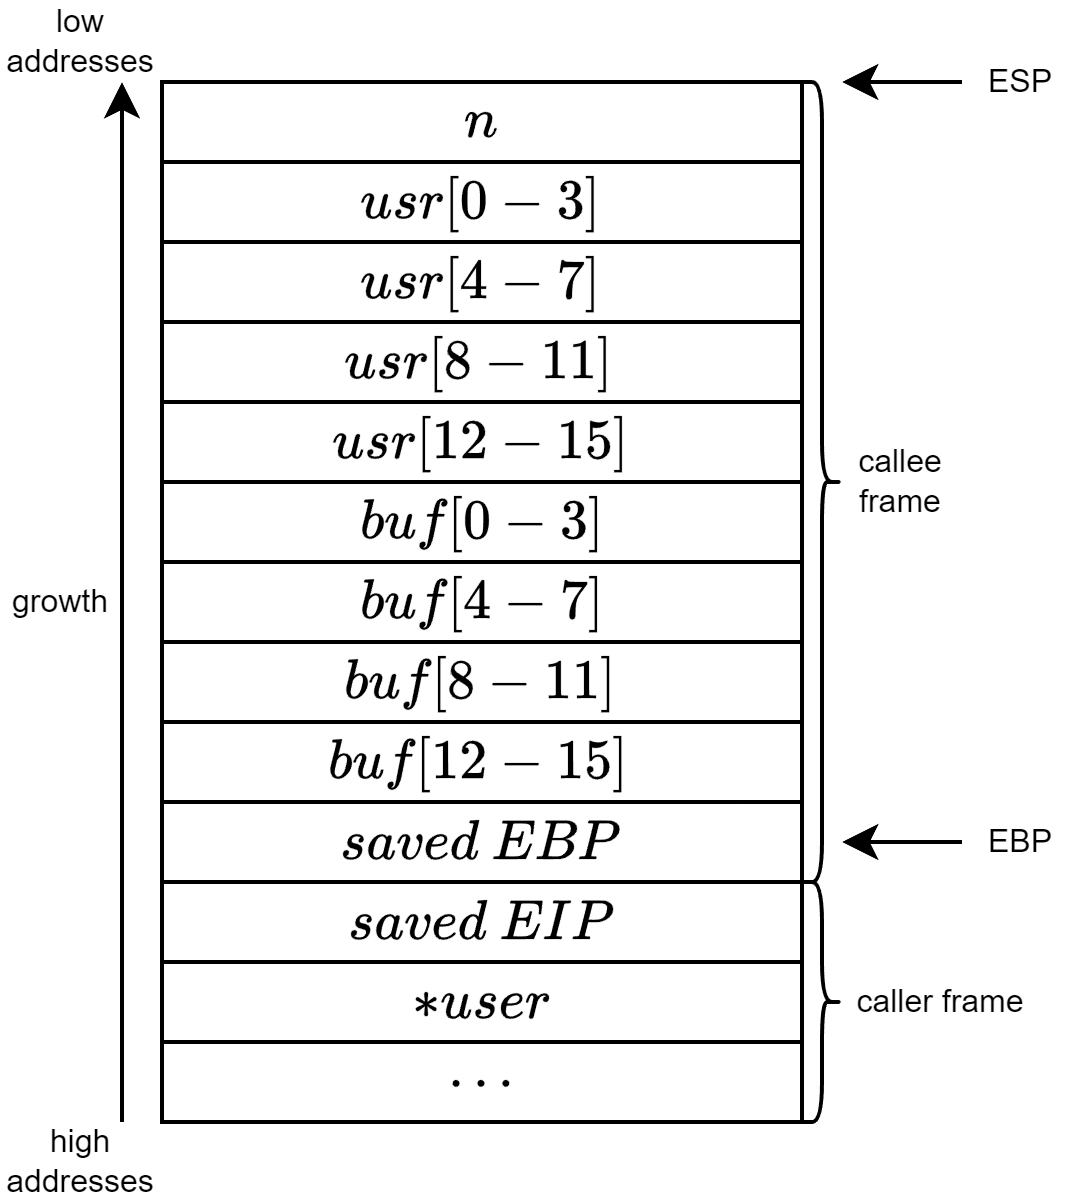
\includegraphics[width=0.5\linewidth]{images/stack6.png}
        \end{figure}
    \item A buffer overflow occurs at line fifteen because \texttt{scanf} reads a user-supplied string of arbitrary length and copies it into a stack buffer.
    \item The stack with the exploit applied is as follows:
        \begin{figure}[H]
            \centering
            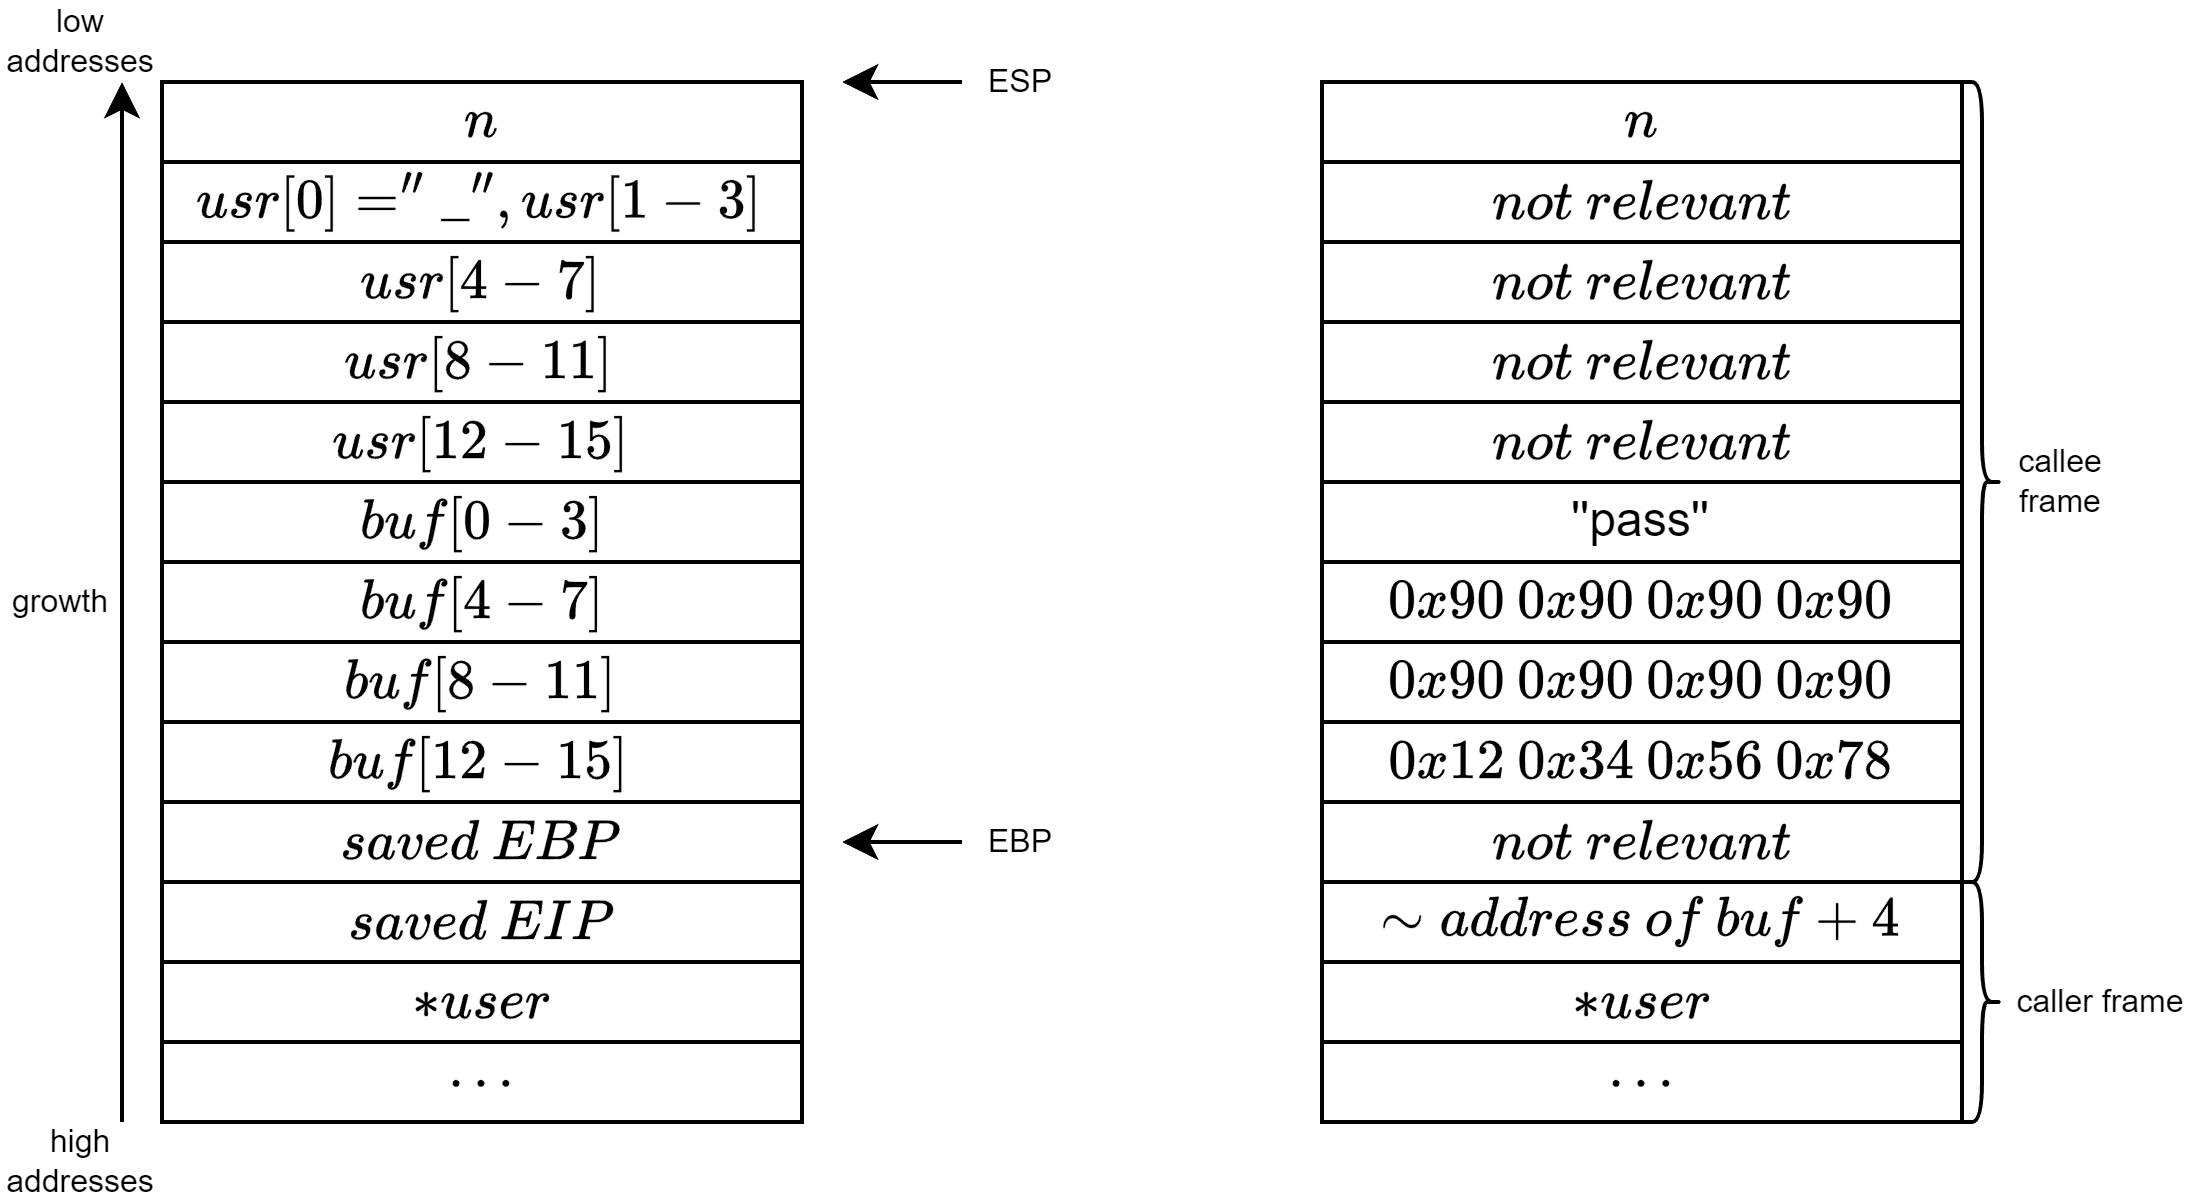
\includegraphics[width=0.75\linewidth]{images/stack7.png}
        \end{figure}
\end{enumerate}